\documentclass{beamer}
\usepackage{verbatim} 
\usepackage{amsthm}
\usepackage{amsmath}
\usepackage{color}
\usepackage{xspace}
\usepackage{bussproofs}
\usepackage{wrapfig}
\usepackage{subfloat}
\usepackage[english]{algorithm2e}

\newcommand{\mypause}{\pause}
%%\newcommand{\mypause}{}
\lefthyphenmin=5
\usepackage{tikz}
%%\usetikzlibrary{arrows,backgrounds,snakes,shapes}

\usepgflibrary{arrows,
               shapes.geometric,
               shapes.symbols,
               shapes.callouts}

\usetikzlibrary{arrows,
                decorations.pathmorphing,
                backgrounds,
                fit,
                shapes.symbols,
                shapes.geometric,
                shapes.callouts,
                through}
\usepackage{graphicx}
\newcommand{\scade}{{\small \sc \textit{SCADE}}}
\newcommand{\scadetitle}{{\sc \textit{SCADE }}}

\tikzstyle{box3}=[draw,thick,text width=1.9cm,text centered,font=\tiny]
\newcommand{\Nat}{{\mathbb N}}
\newcommand{\Real}{{\mathbb R}}
\newcommand{\compatible}[2]{\mathrm{compatible}(#1,#2)}
\newcommand{\incompatible}[2]{\mathrm{incompatible}(#1,#2)}
\newcommand{\success}[3]{\mathrm{success}(#1,#2,#3)}
\newcommand{\consistent}{\mathrm{consistent\,}}
\newcommand{\var}{\mathrm{Var}}
\newcommand{\forallnc}{\forall_{\mathrm{nc}}}
\newcommand{\existsnc}{\exists_{\mathrm{nc}}}
\newcommand{\ire}[2]{#1\,\mathbf{r}\,#2}
\newcommand{\Sub}{\mathbf{Sub}}
\newcommand{\Reso}{\mathbf{Res}}
\newcommand{\Unit}{\mathbf{Unit}}
\newcommand{\Red}{\mathbf{Red}}
\newcommand{\Split}{\mathbf{Split}}
\newcommand{\Elim}{\mathbf{Elim}}
\newcommand{\Conflict}{\mathbf{Conflict}}
\newcommand{\mybar}[1]{\overline{#1}}
\newcommand{\vdashnD}[1]{\overset{#1}{\vdash_{D}}}
\newcommand{\vdashnR}[1]{\overset{#1}{\vdash_{R}}}
\newcommand{\DeltaVec}{\overrightarrow{\Delta}}
\newtheorem{proposition}{Proposition}
\newtheorem{proofbegin}{Proof}
\newtheorem{mylemma}{Lemma}
\newtheorem{myexample}{Example}
\newcommand{\modres}[2]{\overset{#1;#2}{\underset{URes}{\vdash}}}
\newcommand{\UnitSub}{\mathbf{UnitSub}}
\newcommand{\BD}[1]{\mathrm{BD}(#1)}
\newcommand{\DMA}[2]{\mathrm{DMA}(#1,#2)}

\title{Verification of Train Control Systems: Tools and Techniques}
\author[Andy Lawrence]{Andy Lawrence}
\usetheme{Warsaw}
\date{2nd March 2015}


\begin{document}

\begin{frame}
\titlepage

\end{frame}



\begin{frame}
\frametitle{Motivation}
During my Masters of Research I verified \textbf{discrete} railway interlockings using a SAT solver. \\

\medskip

Initially, I decided to try and integrate SAT solving and model checking techniques with our interactive theorem prover Minlog. \\

\medskip

The first step towards this goal is the extraction of the SAT algorithms from constructive proofs. \\

\medskip

I also wanted to see whether model checking could be extended to verify \textbf{continuous} train control systems.

\end{frame}
\begin{comment}
\begin{frame}
\frametitle{Motivation II}
I was set the challenge of modelling the European Rail Traffic Management System by Invensys Rail. \\
\medskip
I formalized ERTMS using hybrid automata to get a grip of the system. \\
\medskip
Subsequently I formalized the pentagon example and a small example junction in Real Time Maude. \\
\medskip
Since the submission of the thesis, I have improved the modelling of the junction and reimplementing it using a general modelling approach. \\
\end{frame}
\end{comment}

\begin{frame}
\frametitle{Extracting DPLL and Resolution Algorithms: Background}
\begin{definition}[Boolean Satisfaction Problem]
Given a formula $\Delta$ is it possible to find a valuation $\Gamma$ such that
 $$\Gamma \models \Delta$$
\end{definition} \hspace*{5pt }\\
\bigskip

The SAT problem is NP complete so all problems in NP can be translated into an instance of the SAT problem.\\
\medskip
This means that SAT-solvers have many applications e.g. Model checking, planning $\ldots$.

\end{frame}

\begin{frame}
\frametitle{Extracting DPLL and Resolution Algorithms: Overview I}

The DPLL proof system consists of 5 rules:


\begin{center}

\AxiomC{$\Gamma, \alert{l} \vdash \Delta $}
\RightLabel{($\Unit$)}
\UnaryInfC{$\Gamma \vdash \Delta, \alert{\{l \}} $}
\DisplayProof \
\AxiomC{$\Gamma, \alert{l} \vdash \Delta, C$}
\RightLabel{($\Red$)}
\UnaryInfC{$\Gamma, \alert{l} \vdash \Delta,  (\alert{\bar{l}}, C)$}
\DisplayProof \

\bigskip

\AxiomC{$\Gamma, \alert{l} \vdash \Delta$}
\RightLabel{($\Elim$)}
\UnaryInfC{$\Gamma, \alert{l} \vdash \Delta,  (\alert{l}, C)$}
\DisplayProof \

\bigskip

\AxiomC{$$}
\RightLabel{($\Conflict$)}
\UnaryInfC{$\Gamma \vdash \Delta,  \alert{\emptyset}$}
\DisplayProof \
\AxiomC{$\Gamma,\alert{l} \vdash \Delta$}
\AxiomC{$\Gamma, \alert{\bar{l}} \vdash \Delta$}
\RightLabel{($\Split$)}
\BinaryInfC{$\Gamma  \vdash \Delta$}
\DisplayProof \


\end{center}
\bigskip

Here $\Delta$ is a formula (clause set) and $\Gamma$  is a valuation (set of literals).
\end{frame}

\begin{frame}
\frametitle{Extracting DPLL and Resolution Algorithms: Overview II}

Skipping some notation and definitions, the expected statement of completeness is:

  $$ \forall \Gamma,\Delta (incompatible(\Gamma; \Delta ) \to \Gamma \vdash \Delta) $$
\pause
I proved the following classically equivalent but constructively
stronger statement:
   $$\forall \Gamma,\Delta (compatible(\Gamma; \Delta) \vee \Gamma \vdash \Delta)$$
 
\pause
The latter statement
yields in addition a model if $\Gamma$ and $\Delta$ are compatible ($\exists M. \, M \models \Gamma \wedge M \models \Delta$).
\end{frame}

\begin{frame}
\frametitle{Extracting DPLL and Resolution Algorithms: Overview III}
\begin{center}
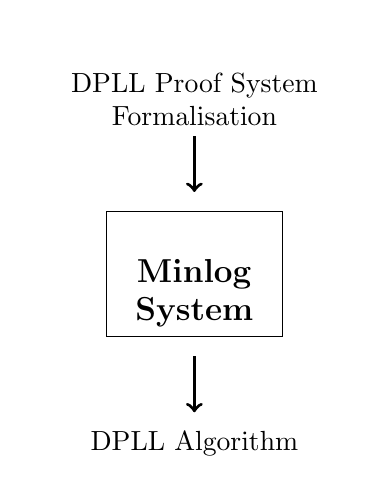
\begin{tikzpicture}[node distance = 3cm]

\tikzstyle{box1}=[rectangle, draw, text width = 1cm, font=\small]
\tikzstyle{box3}=[rectangle, draw, text width = 2cm, font=\large]
\tikzstyle{arrow}=[->,very thick,shorten >=7pt,shorten <=7pt]
\tikzstyle{biarrow}=[<->,very thick,shorten >=7pt,shorten <=7pt]


\node (A) [box3]                   {\begin{center}\textbf{Minlog}\\
					 \textbf{System} \end{center}
                                            };
\draw[arrow] (0,2) -- node[above =10pt, text width = 4cm] {\begin{center} DPLL Proof System Formalisation \end{center}}(A);
\draw[arrow] (A) -- node [below = 13pt] {DPLL Algorithm} (0,-2);
\end{tikzpicture}
\end{center}
\end{frame}

\begin{frame}
\frametitle{Extracting DPLL and Resolution Algorithms: Overview IV}

I have extracted a resolution solver from the proof of the following statement:

$$\forall \Delta. \exists n \, \Delta \vdashnR{n} \emptyset \vee  \exists M. \,  M \models \Delta$$

\bigskip

For all formulae there either is a resolution derivation of size $n$ that it is unsatisfiable or there exists a model of that formula.
\end{frame}

\begin{frame}
\frametitle{Extracting DPLL and Resolution Algorithms: Results}
I extracted a DPLL algorithm that performs reasonably well.\\
\bigskip
\begin{tabular}{|c|c|c|c|c|c|}
  \hline
  \textbf{Formula}  & \textbf{Minlog} &  \multicolumn{2}{|c|}{\textbf{Interpreted (\texttt{ghci})}} & \multicolumn{2}{|c|}{\textbf{Compiled (\texttt{ghc -O2})}}  \\ \hline
  & \textbf{Witness} & \textbf{Witness} & \textbf{Yes/No} & \textbf{Witness} & \textbf{Yes/No} \\ \hline
  PHP(4,3) & 15.32s   &  0.17s   &  0.12s  &  0.008s  &  0.004s \\ \hline
  PHP(4,4) & 6.87s    &  0.08s   &  0.07s  &  0.000s  &  0.000s \\ \hline
  PHP(5,4) & 219.78s  &  1.52s   &  1.08s  &  0.032s  &  0.020s \\ \hline
  PHP(5,5) & 33.15s   &  0.18s   &  0.19s  &  0.004s  &  0.004s \\ \hline
  PHP(6,5) & 2245.27s &  16.68s  &  11.71s &  0.340s  &  0.124s \\ \hline
  PHP(6,6) & 84.88s   &  0.54s   &  0.53s  &  0.012s  &  0.012s \\ \hline
\end{tabular} \\
\bigskip

A resolution solver, based on the DPLL algorithm, was also extracted.

\end{frame}



\begin{frame}
\frametitle{Extracting DPLL and Resolution Algorithms: Publications}
 \begin{thebibliography}{10}    
  \beamertemplatearticlebibitems
\bibitem{AL12a} Lawrence, A. and Berger, U. and Seisenberger, M.
\newblock{\em Extracting a {DPLL} Algorithm} \\
Mathematic Foundations of Program Semantics \\
Electronic Notes in Computer Science \\
Elsevier 2012.
\medskip
\bibitem{AL14b} Berger, U. and Lawrence, A. and Nordvall-Forsberg, F. and Seisenberger, M.
\newblock{\em Extracting Verified Decision Procedures: {DPLL} and Resolution}
Logical Methods in Computer Science, accepted 2014.
\end{thebibliography}
\end{frame}

\begin{frame}
\frametitle{Extracting A CDCL Algorithm: Overview I}
The standard DPLL algorithm can be seen as doing a brute force search for a solution but using unit clauses and heuristics to choose a nice variable ordering.

\medskip

Many modern SAT solvers make use of an optimisation called \alert{clause learning}.

\medskip

Clause learning SAT solvers attempt to reduce the search space by learning clauses during the search.
\medskip

When a clause is learned it may mean that a number of assignments have to be undone which causes \alert{non-chronological backtracking}.


\end{frame}

\begin{frame}
\frametitle{Extracting A CDCL Algorithm: Overview II}

I proved a completeness statement of the following form:
\begin{align*}
 &\forall \Gamma, \Delta. \consistent{\Gamma} \to   \\ 
 &\emptyset \notin \Delta \to \\ 
&( \exists \DeltaVec \, \mathrm{UnitRes}(\DeltaVec_{\delta(\Gamma)} , \Gamma,  \Delta) )\to \\
&\compatible{\Gamma}{\Delta} \vee \exists n \leq \delta(\Gamma) \,    \exists \Delta'  \Gamma_n  \vdash_{\Delta'} \Delta
\end{align*}
$\DeltaVec_{\delta(\Gamma)}$ is a set of formulae $\Delta_0, \ldots, \Delta_{\delta(\Gamma)}$ where each $\Delta_n$ contains the clauses derived from $\Gamma$ by unit resolution at  decision level $n$ starting with $\Delta_0 = \Delta$.
\end{frame}

\begin{frame}
\frametitle{Extracting A CDCL Algorithm: Results}

The following results were achieved:
\begin{enumerate}
\item modified the proof systems that captures the behaviour of clause learning
\item captured non-chronological backtracking at the proof level
\item extracted a prototype clause learning algorithm
\end{enumerate}
\bigskip

Unfortunately there are issues with totality and speed. 
\end{frame}

\begin{frame}

\frametitle{European Rail Traffic Management System (ERTMS)}

What it is:
\begin{itemize}

\item
European standard of signalling, control and train protection 

\item
to replace the many incompatible safety systems currently used by
European railways

\item 
offers possibility for traffic management
\end{itemize}

\bigskip

What it shall achieve:
\begin{itemize}

\item 
interoperability

\item
ease of maintenance (less track equipment)

\item 
higher capacity

\end{itemize}

\end{frame}

\begin{frame}
\frametitle{ERTMS Information Flow}
\begin{center}
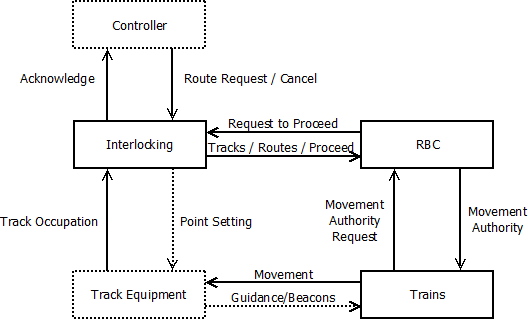
\includegraphics[scale=0.5]{wadtsiemens.png}
\end{center}
\end{frame}


\begin{frame}
\frametitle{Modelling and Verifying ERTMS: Train Automaton}

\begin{center}
\scalebox{0.6}{
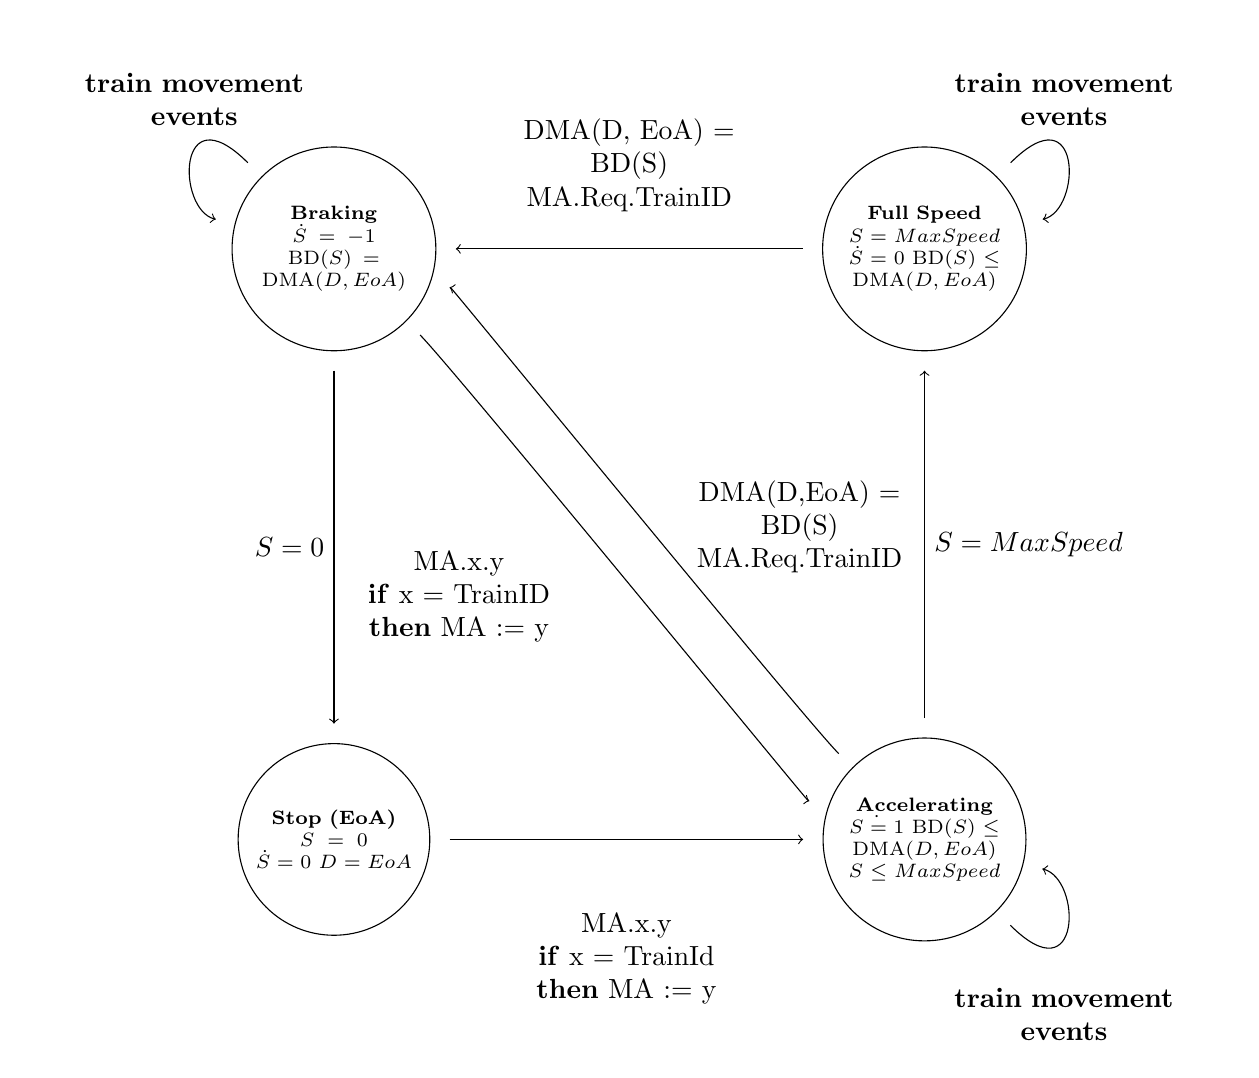
\begin{tikzpicture}[node distance = 2cm]

\tikzstyle{box1}=[circle, draw, text width = 2cm, font=\scriptsize, text centered]
\tikzstyle{arrow}=[->,shorten >=7pt,shorten <= 7pt]
\tikzstyle{biarrow}=[<->,very thick,shorten >=7pt,shorten <=7pt]


\node (A) [box1]  at (0,0)                  {\textbf{Stop (EoA)} \\
							$S = 0$ \\
                                                        $\dot{S} = 0$
							$D = EoA$ 

                                            };

\node (B) [box1]    at (7.5,0)          { \textbf{Accelerating} \\
       $\dot{S = 1}$
       $\BD{S} \leq \DMA{D}{EoA}$
       $S \leq MaxSpeed$
};

\node (C)[box1] at (0, 7.5)  { \textbf{Braking}\\
					                   $\dot{S} = -1$ 
						           $\BD{S} = \DMA{D}{EoA}$
                                               
						};

\node (D)[box1] at (7.5, 7.5)  { \textbf{Full Speed }\\
					                   $S = MaxSpeed$
                                                            $\dot{S} = 0$
							    $\BD{S} \leq \DMA{D}{EoA}$             
						};


\draw [arrow] (B) -- node[right] {$S = MaxSpeed$} (D);
\draw [arrow] (A) -- node[below = 10pt, text width = 4cm] {\begin{center}MA.x.y\\ \textbf{if} x = TrainId\\ \textbf{then} MA := y\end{center} } (B);
\draw [arrow] (D) --  node[above = 10pt,text width=4cm] {\begin{center}DMA(D, EoA) =\\ BD(S)\\MA.Req.TrainID \end{center}} (C);
\draw [arrow] (C) -- node [left] {$S = 0$} (A);
\draw [arrow] (B)  .. controls +(-1.5cm,  1.5 cm) and +(1.5cm,  -0.5 cm ) .. node [right,text width=4cm] { \begin{center}DMA(D,EoA) =\\
    BD(S)\\MA.Req.TrainID \end{center}} (C);
\draw [arrow] (C) .. controls +(1.5cm,  -1.5cm) and +(-1.5cm, 0.5 cm ) ..   node [left,text width = 4cm] {\begin{center}MA.x.y\\ \textbf{if} x = TrainID \\ \textbf{then} MA := y\end{center} } (B);
\draw [arrow] (C) .. controls +(-2cm,  2cm) and +(-2cm, 0.5 cm ) ..   node [above = 10pt, text width = 4cm] {\begin{center}\textbf{train movement events} \end{center}} (C);
\draw [arrow] (D) .. controls +(2cm,  2cm) and +(2cm, 0.5 cm ) ..   node [above = 10pt, text width = 4cm] {\begin{center} \textbf{train movement events} \end{center}} (D);
\draw [arrow] (B) .. controls +(2cm,  -2cm) and +(2cm, -0.5 cm ) ..   node [below = 6pt, text width = 4cm] {\begin{center}\textbf{train movement events} \end{center}} (B);

\end{tikzpicture}
}  
\end{center}
\end{frame}

\begin{frame}
\frametitle{Modelling and Verifying ERTMS: RBC Automaton}

\begin{center}
\scalebox{0.6}{
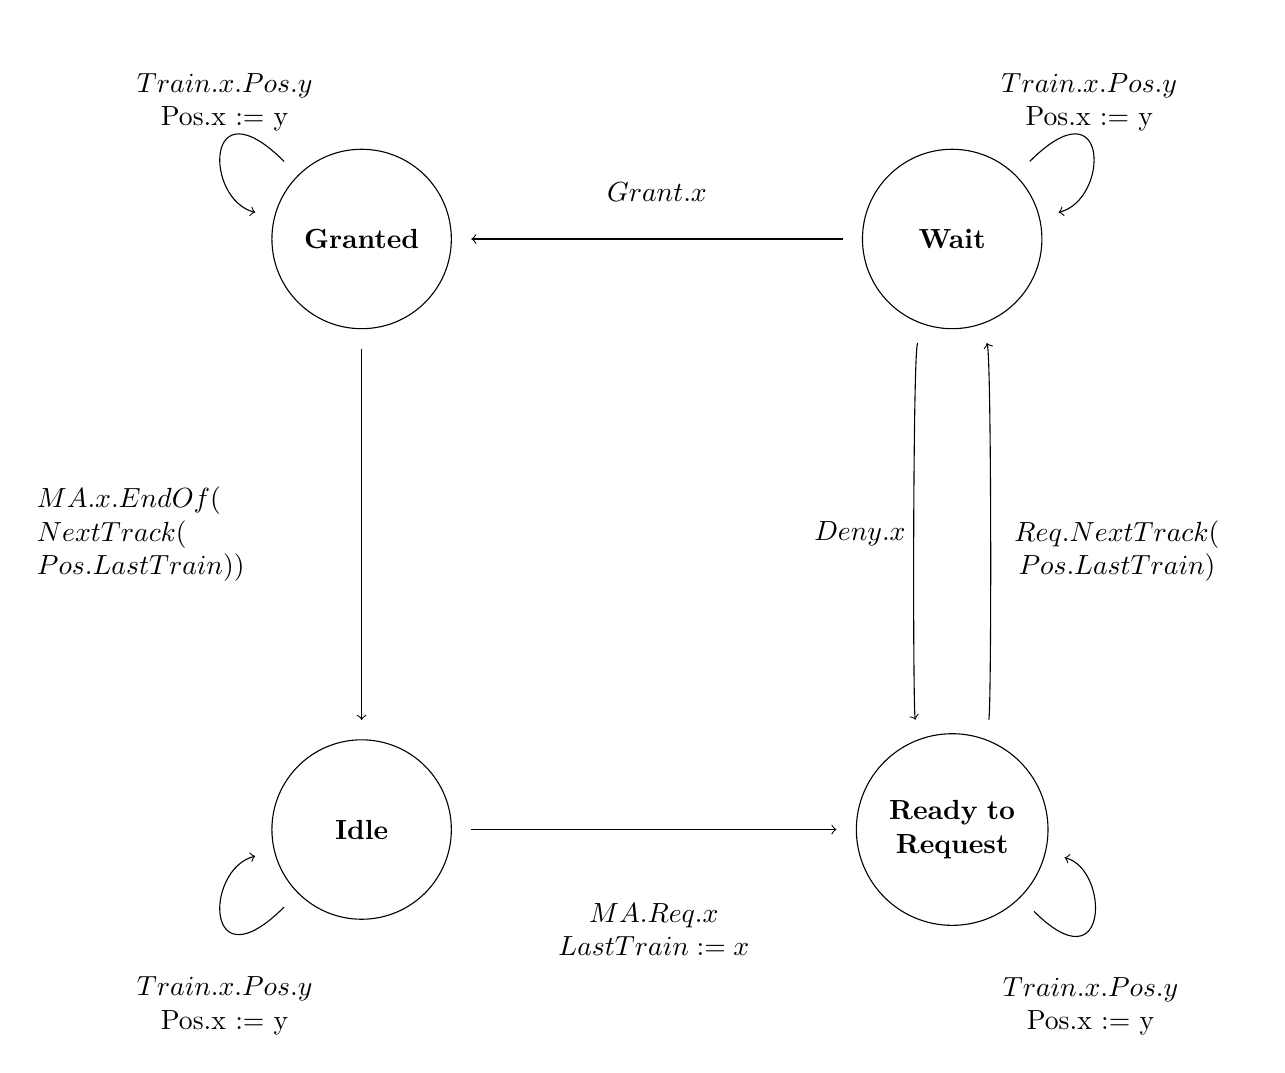
\begin{tikzpicture}[node distance = 1cm]
\tikzstyle{box1}=[circle, draw, text width = 2cm, text centered ]
\tikzstyle{arrow}=[->,shorten >=7pt,shorten <= 7pt]
\tikzstyle{biarrow}=[<->,very thick,shorten >=7pt,shorten <=7pt]
\node (A) [box1]  at (0,0)                  {\textbf{Idle} };
\node (B) [box1]    at (7.5,0)          {\textbf{Ready to Request} };
\node (C)[box1] at (0, 7.5)  {  \textbf{Granted}  };
\node (D)[box1] at (7.5, 7.5)  { \textbf{Wait} };


\draw [arrow] (B)  .. controls +(0.5cm,  1.5 cm) and +(0.5cm,  -1.5 cm ) .. node[right, text width = 3cm] {\begin{center}$Req.NextTrack($ \\ $Pos.LastTrain)$ \end{center}} (D);
\draw [arrow] (D) .. controls +(-0.5cm,  -1.5cm) and +(-0.5cm, 1.5 cm ) ..   node [left] {$Deny.x$} (B);
\draw [arrow] (A) -- node[below = 10pt, text width = 4cm] {\begin{center}$MA.Req.x$ \\ $LastTrain := x$\end{center}} (B);
\draw [arrow] (D) --  node[above = 10pt,text width=4cm] {\begin{center}$Grant.x$\end{center}} (C);
\draw [arrow] (C) -- node [left, text width = 4cm] {$MA.x.EndOf($ \\ $NextTrack($ \\ $Pos.LastTrain))$} (A);

\draw [arrow] (C) .. controls +(-2cm,  2cm) and +(-2cm, 0.5 cm ) ..   node [above = 5pt, text width = 4cm] {\begin{center}$Train.x.Pos.y$\\ Pos.x := y\end{center}} (C);
\draw [arrow] (D) .. controls +(2cm,  2cm) and +(2cm, 0.5 cm ) ..   node [above = 5pt, text width = 4cm] {\begin{center}$Train.x.Pos.y$\\ Pos.x := y\end{center}} (D);
\draw [arrow] (B) .. controls +(2cm,  -2cm) and +(2cm, -0.5 cm ) ..   node [below = 6pt, text width = 4cm] {\begin{center}$Train.x.Pos.y$\\ Pos.x := y\end{center}} (B);
\draw [arrow] (A) .. controls +(-2cm,  -2cm) and +(-2cm, -0.5 cm ) ..   node [below = 6pt, text width = 4cm] {\begin{center}$Train.x.Pos.y$\\ Pos.x := y\end{center}} (A);


\end{tikzpicture} 
}
\end{center}

\end{frame}

\begin{frame}
\frametitle{Modelling and Verifying ERTMS: Interlocking Automaton}

\begin{center}
\scalebox{0.7}{
\begin{tikzpicture}[scale = 0.6]

\tikzstyle{box1}=[circle, draw, text width =3cm,text centered]
\tikzstyle{arrow}=[->,shorten >=7pt,shorten <= 7pt]
\tikzstyle{biarrow}=[<->,very thick,shorten >=7pt,shorten <=7pt]



\node (B) [box1]    at (7.5,0)          {\textbf{Idle}

};

\node (C)[box1] at (0, 7.5)  {\textbf{Response}                                             
						};

\draw [arrow] (B)  .. controls +(-1.5 cm,  2.75 cm) and +(4.5cm,  -2.5cm ) .. node [right, text width=4cm] {Req.z} (C);
\draw [arrow] (C) .. controls +(1cm,  -3cm) and +(-2.75cm, 1 cm ) ..   node [left = 3 cm, below, text width = 6cm] {$Grant.z \  \mathbf{if} \ t_{ReqId} = \ free $\\$ \mathbf{else} \ Deny.z \ Otherwise$} (B);


\end{tikzpicture}
} 
\end{center}
\end{frame}

\begin{frame}
\frametitle{Modelling and Verifying ERTMS: Examples}

\begin{center}
\begin{tabular}{cc}
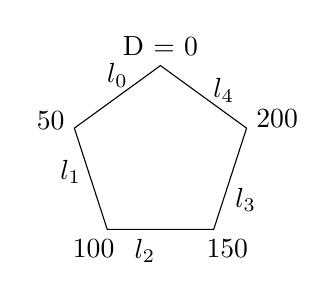
\begin{tikzpicture}[node distance = 2.3cm, scale = 0.7]
\node (A) [draw,regular polygon, regular polygon sides=5, minimum size=2.3 cm,outer sep=0pt] {};
\foreach \n in {1,...,1} {
    \pgfmathtruncatemacro{\value}{(\n - 1) * 50};
    \pgfmathtruncatemacro{\valuem}{(\n - 1)};
    \node at (A.corner \n) [anchor=360/5*(\n-1)+270] {D = \value};
    \node at (A.side \n) [anchor = 360/5 *(\n-1) +270] {$l_{\valuem}$};
}
\foreach \n in {2,...,5} {

    \pgfmathtruncatemacro{\value}{(\n - 1) * 50};
    \pgfmathtruncatemacro{\valuem}{(\n - 1)};
    \node at (A.corner \n) [anchor=360/5*(\n-1)+270] { \value};
    \node at (A.side \n) [anchor = 360/5 *(\n-1) +270] {$l_{\valuem}$};
}
%%%\node (B) [draw, rectangle, rotate = 36] at (-1.9,2.6) {Train A};
%%%\node (C) [draw, rectangle, rotate =72] at (3,-1) {Train B};
\end{tikzpicture} &
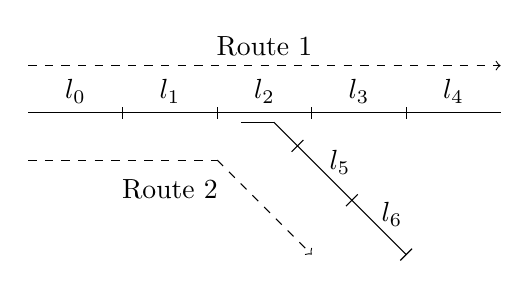
\begin{tikzpicture}[node distance = 3cm, scale = 0.6]
\draw (0,0) -- (10,0);
\foreach \n in {1,...,5} {
  \pgfmathtruncatemacro{\valuem}{(\n - 1)};
    \node () [above] at (\n *2 -1,0) {$l_{\valuem}$};
}
\foreach \n in {2,...,5} {
  \pgfmathtruncatemacro{\valuem}{(\n - 1)};
    \draw (\valuem *2, -0.125) -- (\valuem *2, 0.125) ;
}
\draw (4.5,-0.2) -- (5.2, -0.2);
\draw (5.2,-0.2) -- (8,-3);
\draw (5.575,-0.825) -- (5.825,-0.575);
\draw (6.725,-1.975) -- (6.975,-1.725);
\draw (8.125,-2.875) -- (7.875, -3.125);
\node () [] at (6.6,-1.05) {$l_5$};
\node () [] at (7.7,-2.15) {$l_6$};
\draw [->,dashed] (0,1) -- (10,1);
\node () [above] at (5,1) {Route 1};
\draw[dashed] (0,-1) -- (4,-1);
\draw[->,dashed] (4,-1) -- (6,-3);
\node() [below] at (3,-1.2) {Route 2};
\end{tikzpicture} 
 \\
Pentagon-Example & Junction
\end{tabular}
\end{center}

\end{frame}



\begin{frame}
\frametitle{Modelling and Verifying ERTMS: Results}
This model enables us to: 
\begin{enumerate}
\item analyse and verify quantitative properties such as capacity and performance
\item verify qualitative properties such as safety
\end{enumerate}
\bigskip
The railway industry aims to increase capacity whilst maintaining safety.
\end{frame}

\begin{frame}
\frametitle{Simulation via Execution of the Specification: Train1 Graph}
\begin{center}
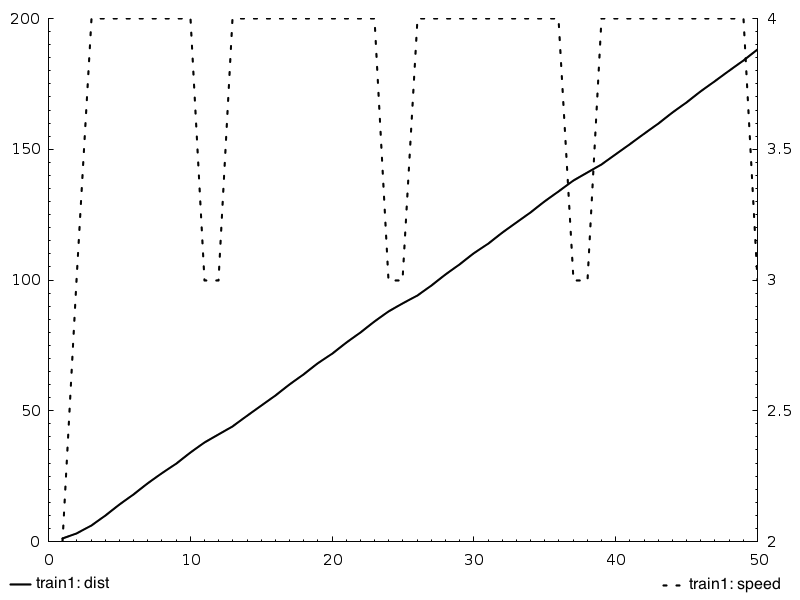
\includegraphics[scale=0.3]{t1graph.png}
\end{center}
\end{frame}

\begin{frame}
\frametitle{Simulation via Execution of the Specification: Train2 Graph}
\begin{center}
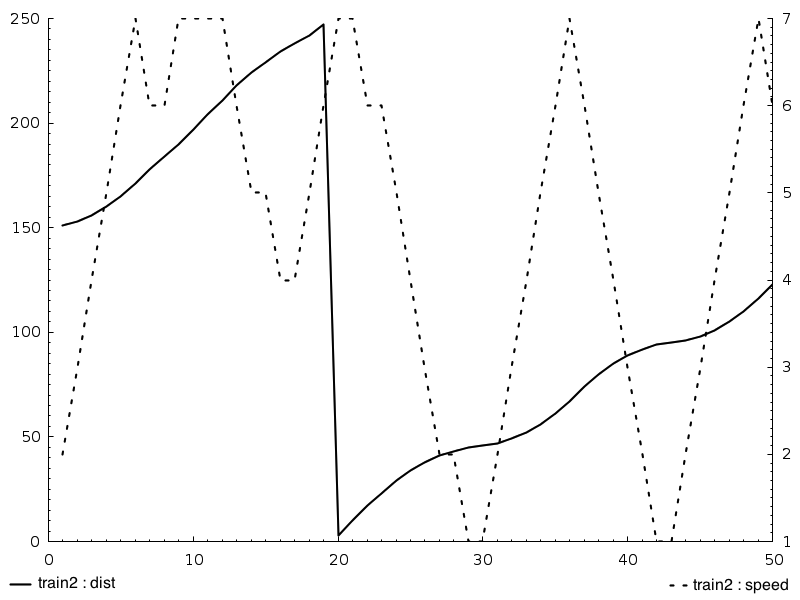
\includegraphics[scale=0.3]{t2graph.png}
\end{center}
\end{frame}



\begin{frame}
\frametitle{Safety-Verification by applying Real-Time Maude
  Model-checking for Linear Temporal Logic}

Pentagon Example - 2 trains:
\begin{itemize}
\item
no overlapping MA in the first 100 time units
-- takes 91 secs
\end{itemize}

\bigskip
%Pentagon Example - 2 trains - tracklength 5000 - speed 120/70
%\begin{itemize}
%\item
%no overlapping MA in the first 70 time units
%-- takes 79 secs
%\end{itemize}

%\bigskip\bigskip

Junction - 2 trains:
\begin{itemize}
\item
no overlapping MA -- takes 7 secs

\item 
no derailment  -- takes 6 secs

\end{itemize}

\pause
\bigskip

I also compared this with realistic track segment lengths of 5000 - speed 120/70

\medskip

Pentagon Example - 2 trains:
\begin{itemize}
\item
no overlapping MA in the first 70 time units -- takes 79 secs
\end{itemize}
\end{frame}


\begin{frame}
\frametitle{Modelling and Verifying ERTMS: Publications}
 \begin{thebibliography}{10}    
  \beamertemplatearticlebibitems
\bibitem{AL14c} Berger, U. and Lawrence, A. and Roggenbach, M. and Seisenberger, M.
\newblock{\em Safety and Performance of the European Rail Traffic Management System: A Modelling and Verification Exercise in Real Time Maude} \\
WADT, 2014.
\medskip
\bibitem{AL12a} Berger, U. and James, P. and Lawrence, A. and Roggenbach, M. and
	Seisenberger, M.
\newblock{\em Modelling and Analysing the European Rail Traffic Management System
	in Real Time Maude} \\
FTSCS, 2014.
\end{thebibliography}
\end{frame}

\begin{frame}
\frametitle{Modelling and Verifying ERTMS: Future Work}
We plan to submit a journal paper with the following improvements:
\begin{enumerate}
\item A generic modelling approach

\item A larger example e.g. a run through station

\end{enumerate}
\medskip
This paper is due April 2015.

\end{frame}

\end{document}
